% Point to the main file
\documentclass[../../Main.tex]{subfiles}

% ========== Start the document ==========
\begin{document}

\section{Section 6.1 - Intro to Counting}

There are 2 highways from Palm Springs to Upland and 3 highways from Upland to Corona. How many ways can one travel from palm Springs to Corona if you must travel through Upland

\begin{center}
    \begin{tabular}{ c|c|c| } 
        & PU1 & PU2 \\
        \hline
        UC1 & & \\
        \hline 
        UC2 & & \\
        \hline 
        UC3 & & \\ 
        \hline
        \end{tabular}
\end{center}

$$2 \cdot 3 = 6 \text{ ways}$$

This is the fundamental theorem of Counting

\begin{theorem}[Fundamental Theorem of Counting]
    If there are $a$ ways to do task A and $b$ was of doing task B, then there are $a \cdot b$ ways to do task A and B
\end{theorem}

\begin{example}

    Let's do some example of this

    \begin{enumerate}
        \item
        {
            How many 2 letter initials are there if...

            \begin{alphabet}
                \item
                {
                    The letters can be repeated?

                    \begin{align*}
                        \underbrace{\underline{26}}_{\text{Letter 1}} \cdot \underbrace{\underline{26}}_{\text{Letter 2}} = \boxed{676}
                    \end{align*}
                }

                \item
                {
                    The letters CANNOT be repeated?

                    \begin{align*}
                        \underbrace{\underline{26}}_{\text{Letter 1}} \cdot \underbrace{\underline{25}}_{\text{Letter 2}} = \boxed{650}
                    \end{align*}

                    Since we can choose any letter for the first one, but the last one we can choose all but the one we just chose, so $26 - 1 = 25$
                }
            \end{alphabet}
        }

        \item
        {
            How many 7 digit phone numbers do not start with 0 or 1?

            \begin{align*}
                \underline{8} \cdot \underline{10} \cdot \underline{10} \cdot \underline{10} \cdot \underline{10} \cdot \underline{10} \cdot \underline{10} = \boxed{8,000,000}
            \end{align*}
        }

        \item
        {
            How many ways can 7 people line up for a picture?

            \begin{alphabet}
                \item 
                {
                    There are no restrictions

                    $$\underline{7} \cdot \underline{6} \cdot \underline{5} \cdot \underline{4} \cdot \underline{3} \cdot \underline{2} \cdot \underline{1} = 7! = \boxed{5040}$$
                }

                \item
                {
                    Dina must be the first person in the photo

                    $$\underline{1} \cdot \underline{6} \cdot \underline{5} \cdot \underline{4} \cdot \underline{3} \cdot \underline{2} \cdot \underline{1} = 6! = \boxed{720}$$
                }

                \item
                {
                    Dina is NOT the first person in the photo

                    $$\underline{6} \cdot \underline{6} \cdot \underline{5} \cdot \underline{4} \cdot \underline{3} \cdot \underline{2} \cdot \underline{1} = 6 \cdot 6! = \boxed{4320}$$

                    OR

                    \begin{align*}
                        \text{\# ways Dina w/ first } + \text{ \# ways Dina NOT first } &= \text{total} \\
                        \text{ \# ways Dina NOT first } &= \text{total} - \text{ \# ways Dina w/ first } \\
                        &= 5040 - 720 \\
                        &= \boxed{4320}
                    \end{align*}
                }

                \item 
                {
                    Dina must stand next to Omar

                    We do this by treating Dina and Omar as one pair

                    But since there's, two ways of arranging Dina and Omar, Dina -> Omar and Omar -> Dina, we gotta multiply it every twice

                    $$2 \left( \underline{6} \cdot \underline{5} \cdot \underline{4} \cdot \underline{3} \cdot \underline{2} \cdot \underline{1} \right) = 2 \cdot 6! = \boxed{1440}$$
                }

                \item
                {
                    Dina must not stand next to Omar

                    \begin{align*}
                        \text{\# Dina next to Omar} + \text{\# Dina NOT next to Omar} &= \text{total} \\
                        \text{\# Dina NOT next to Omar} &= \text{total} - \text{\# Dina next to Omar} \\
                        &= 5040 - 1440 \\
                        &= \boxed{3600} \\
                    \end{align*}
                }
            \end{alphabet}
        }

        \item 
        {
            A bit string is a sequence of $0$'s and $1$'s. How many bit strings are there of length 7?

            \begin{alphabet}
                \item
                {
                    If there are no restrictions

                    $$\underline{2} \cdot \underline{2} \cdot \underline{2} \cdot \underline{2} \cdot \underline{2} \cdot \underline{2} \cdot \underline{2} = 2^7 = \boxed{128} $$
                }

                \item
                {
                    Begin with $01$

                    $$\underline{1} \cdot \underline{1} \cdot \underline{2} \cdot \underline{2} \cdot \underline{2} \cdot \underline{2} \cdot \underline{2} = 2^5 = \boxed{32}$$

                    We could also just say how many ways can we arrange a 5 length bit string since the first two are fixed ($01$)
                } 

                \item
                {
                    Are palindromes, ie are the same when written forwards or backwards

                    $$\underbrace{\underline{2} \cdot \underline{2} \cdot \underline{2} \cdot \underline{2}}_{\text{anything}} \cdot \underbrace{\underline{1} \cdot \underline{1} \cdot \underline{1}}_{\text{fixed}} = 2^4 = \boxed{16}$$
                }
            \end{alphabet}
        }

        \item
        {
            How many ways can 5 people order a single scoops of icecream if the possible flavors are vanilla, coffee, chocolate, strawberry, or olive?

            $$\underline{5} \cdot \underline{5} \cdot \underline{5} \cdot \underline{5} \cdot \underline{5} = 5^5 = \boxed{3125}$$

            Since there's 5 flavors and 5 people
        }

        \item 
        {
            How many whole numbers less than 100 are...

            \begin{alphabet}
                \item 
                {
                    Divisible by 3

                    $$\left\lfloor \frac{100}{3} \right\rfloor = 33 \text{\# of possible ints div by 3}$$

                    $$\left\lfloor \frac{100}{3} \right\rfloor + \underbrace{1}_{\text{including 0}} = \boxed{34}$$
                }

                \item
                {
                    div by 7?

                    $$\left\lfloor \frac{100}{7} \right\rfloor + 1 = 14 + 1 = \boxed{15}$$
                }

                \item
                {
                    div by 3 OR 7?

                    This represents 3 OR 7, where A is all numbes div by 3 and B is same but for 7

                    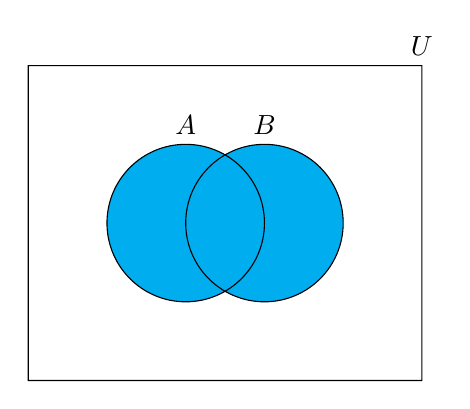
\begin{tikzpicture}[fill=cyan]
                    % left hand
                    \scope
                    \clip (-2,-2) rectangle (2,2)
                        (1,0) circle (1);
                    \fill (0,0) circle (1);
                    \endscope
                    % right hand
                    \scope
                    \clip (-2,-2) rectangle (2,2);
                    \fill (1,0) circle (1);
                    \endscope
                    % outline
                    \draw (0,0) circle (1) (0,1)  node [text=black,above] {$A$}
                        (1,0) circle (1) (1,1)  node [text=black,above] {$B$}
                        (-2,-2) rectangle (3,2) node [text=black,above] {$U$};
                    \end{tikzpicture}

                    This represents div by BOTH 3 and 7

                    
                    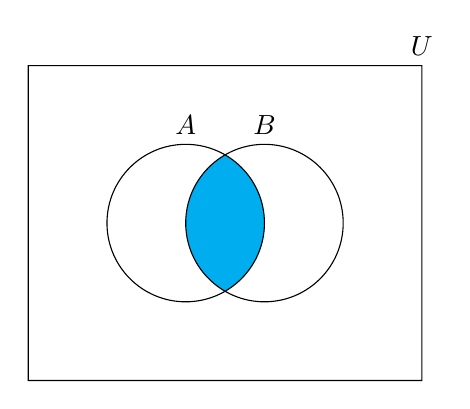
\begin{tikzpicture}[fill=cyan]
                    \scope

                    \clip (-2,-2) rectangle (2,2)
                        (1,0) circle (1)
                        (0,0) circle (1);
                    \fill (0,0) circle (1);

                    \endscope

                    % outline
                    \draw (0,0) circle (1) (0,1)  node [text=black,above] {$A$}
                        (1,0) circle (1) (1,1)  node [text=black,above] {$B$}
                        (-2,-2) rectangle (3,2) node [text=black,above] {$U$};
                    \end{tikzpicture}

                    \begin{recall}
                        $$A \cup B = A + B - A \cap B$$
                    \end{recall}

                    Being divisible by both 3 and 7 just means being divisible by 21

                    $$A \cap B = \left\lfloor \frac{100}{3 \cdot 7} \right\rfloor + 1 = 4 + 1 = 5$$

                    \begin{align*}
                        \mid A \cup B \mid &= \mid A \mid + \mid B \mid - \mid A \cap B \mid \\
                        &= 34 + 15 - 5 \\
                        &= \boxed{44} \\
                    \end{align*}
                }
            \end{alphabet}
        }

        \item
        {
            A die is rolled 5 times. How many wys can this happen if...

            \begin{alphabet}
                \item
                {
                    No restrictions
                    
                    $$\underline{6} \cdot \underline{6} \cdot \underline{6} \cdot \underline{6} = 6^5 = \boxed{7776}$$
                }

                \item
                {
                    4 is never rolled

                    $$\underline{5} \cdot \underline{5} \cdot \underline{5} \cdot \underline{5} \cdot \underline{5} = 5^5 = \boxed{3125}$$
                }

                \item
                {
                    The number 4 is rolled at least once

                    \begin{align*}
                        \text{\# ways 4 is rolled at least once} + \text{\# never rolled} &= \text{total} \\
                        \text{\# ways 4 is rolled at least once} &= \text{total} - \text{\# never rolled} \\
                        &= 7776 - 3125 \\
                        &= 6^5 - 5^5 \\
                        &= \boxed{4651} \\
                    \end{align*}
                }

            \end{alphabet}
        }

        \item
        {
            A pair of dice is rolled. How many outcomes are possible if... 

            \begin{alphabet}
                \item
                {
                    No restrictions
                    
                    $$\underline{6} \cdot \underline{6} = \boxed{36}$$
                }

                \item
                {
                    The sum is 4

                    $$(1, 3), (3, 1), (2, 2)$$ so 3 ways
                }
            \end{alphabet}
        }

        \item
        {
            A coin is flipped 10 times. How many outcomes are possible if

            \begin{alphabet}
                \item
                {
                    No restrictions

                    $$\underline{2} \cdot \underline{2} \cdot  \underline{2} \cdot  \underline{2} \cdot  \underline{2} \cdot  \underline{2} \cdot  \underline{2} \cdot  \underline{2} \cdot  \underline{2} \cdot  \underline{2} = 2^{10} = \boxed{1024}$$
                }

                \item 
                {
                    At least 1 of the flips is heads
                    
                    \begin{align*}
                        \text{\# ways no heads} + \text{\# ways at least 1} &= \text{total} \\
                        \text{\# at least 1} &= \text{total} - \underbrace{\text{\# ways no heads}}_{\text{all tails}} \\
                        &= 2^{10} - 1 \\
                        &= \boxed{1023}
                    \end{align*}
                }
            \end{alphabet}
        }
    \end{enumerate}
    
\end{example}

\subsection{Multiples of n up to k}

\begin{theorem}[Number of Multiples of n up to k]
    To find the number of positive integers divisible by $n$ up to $k$ is given by

    $$\left\lfloor \frac{k}{n} \right\rfloor$$

    This DOES NOT include 0, so for all whole numbers it would be

    $$\left\lfloor \frac{k}{n} \right\rfloor + 1$$
\end{theorem}

% ========== End the document ==========
\end{document}